
\chapter{Simulation Procedure}

  \section{First Runs}

  \section{Choosing the Resolution of the 2D1D-Grid}
    \begin{figure}[h!]
      \centering
      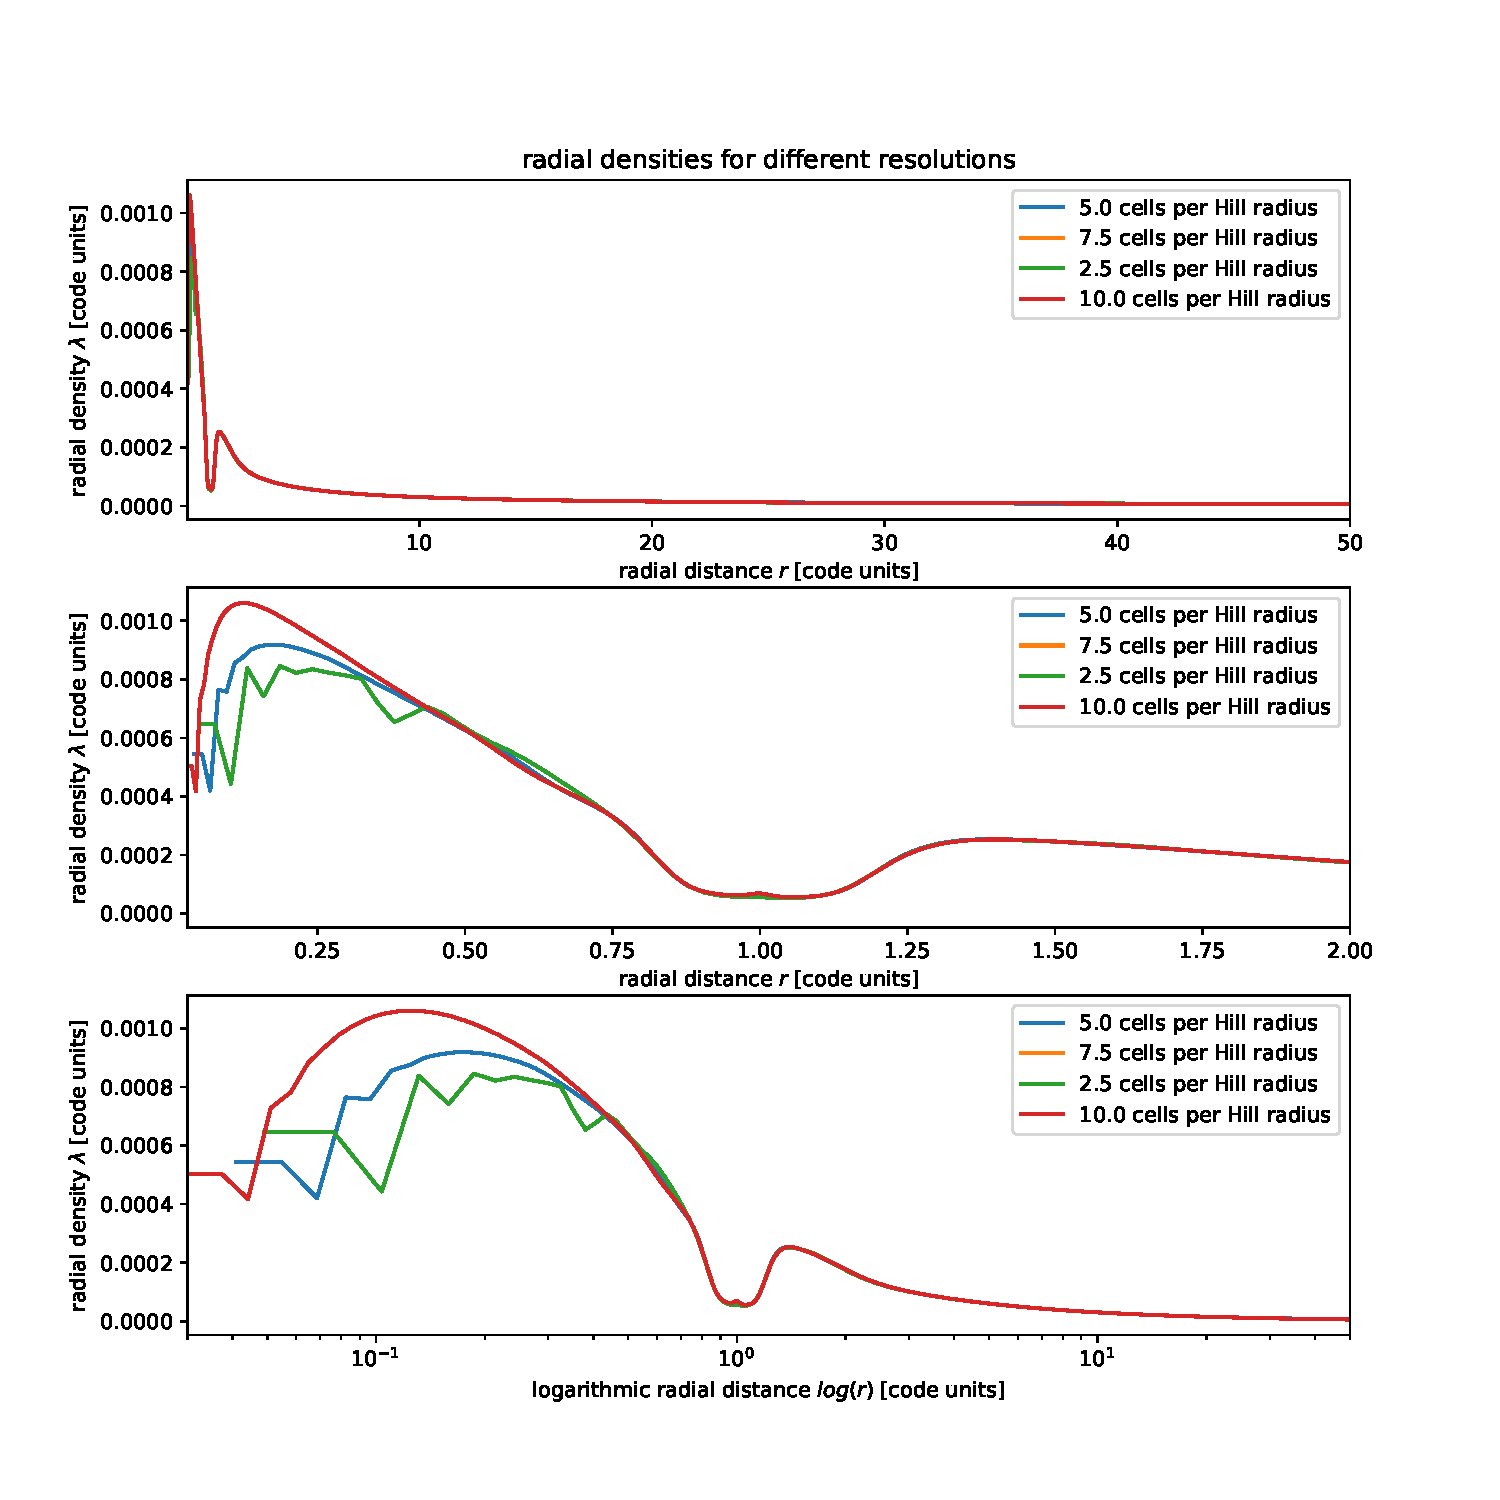
\includegraphics[width=\textwidth]{testing_cells_per_rH/radial_densities_by_resolution.pdf}
      \caption{radial densities after 500 orbits for different resolutions}
      \label{}
    \end{figure} \ \\ 

  \section{Variation of the Parameters of the Protoplanetary Disk}

%    \subsection{Aspect Ratio}

%    \subsection{Viscosity Parameter of the Gas in the Disk}

%    \subsection{Radial Gas Distribution in the Disk}

  \section{Variation of the Initial Parameters of the Planet}

%    \subsection{Initial Mass}

%    \subsection{Eccentricity of the Orbit}

%    \subsection{Machida Accretion Factor}

